\label{sampling_case_study}
The following case study illustrates how the functionality of the \code{inversion}, \code{grabsample} and \code{uq} subcommands 
can be used in tandem to identify multiple sampling cycles that reduce uncertainty in the extent of contamination.
The approach uses successive measurements obtained from manual grab samples to find the contamination plume.  
Figure \ref{fig:ureduction_flowchart} illustrates the methodology.
A contamination incident is first suspected following a customer inquiry or detection from a fixed continuous 
sensor in the Contamination Warning System (CWS). 
At this stage, a team is sent out to gather manual grab samples at and around the location of first detection. 
Discrete yes/no measurements from these manual grab samples along with the measurement from contamination warning system 
are then used to estimate the probability that nodes in the network are contaminated.
The probability of node contamination provides a metric of uncertainty quantification. Given a particular confidence level (e.g., 95\%), 
nodes can be categorized according to their probability of contamination: LY for ``likely yes,'' LN for ``likely no'' and UN for ``unknown.''  

If a sufficiently small number of nodes remain uncertain, then the process is terminated, otherwise further sampling cycles are required. 
This cycle of collecting manual grab samples is continued until the contamination plume is estimated with a good level of confidence. 
\begin{figure}[!ht]
\begin{center}
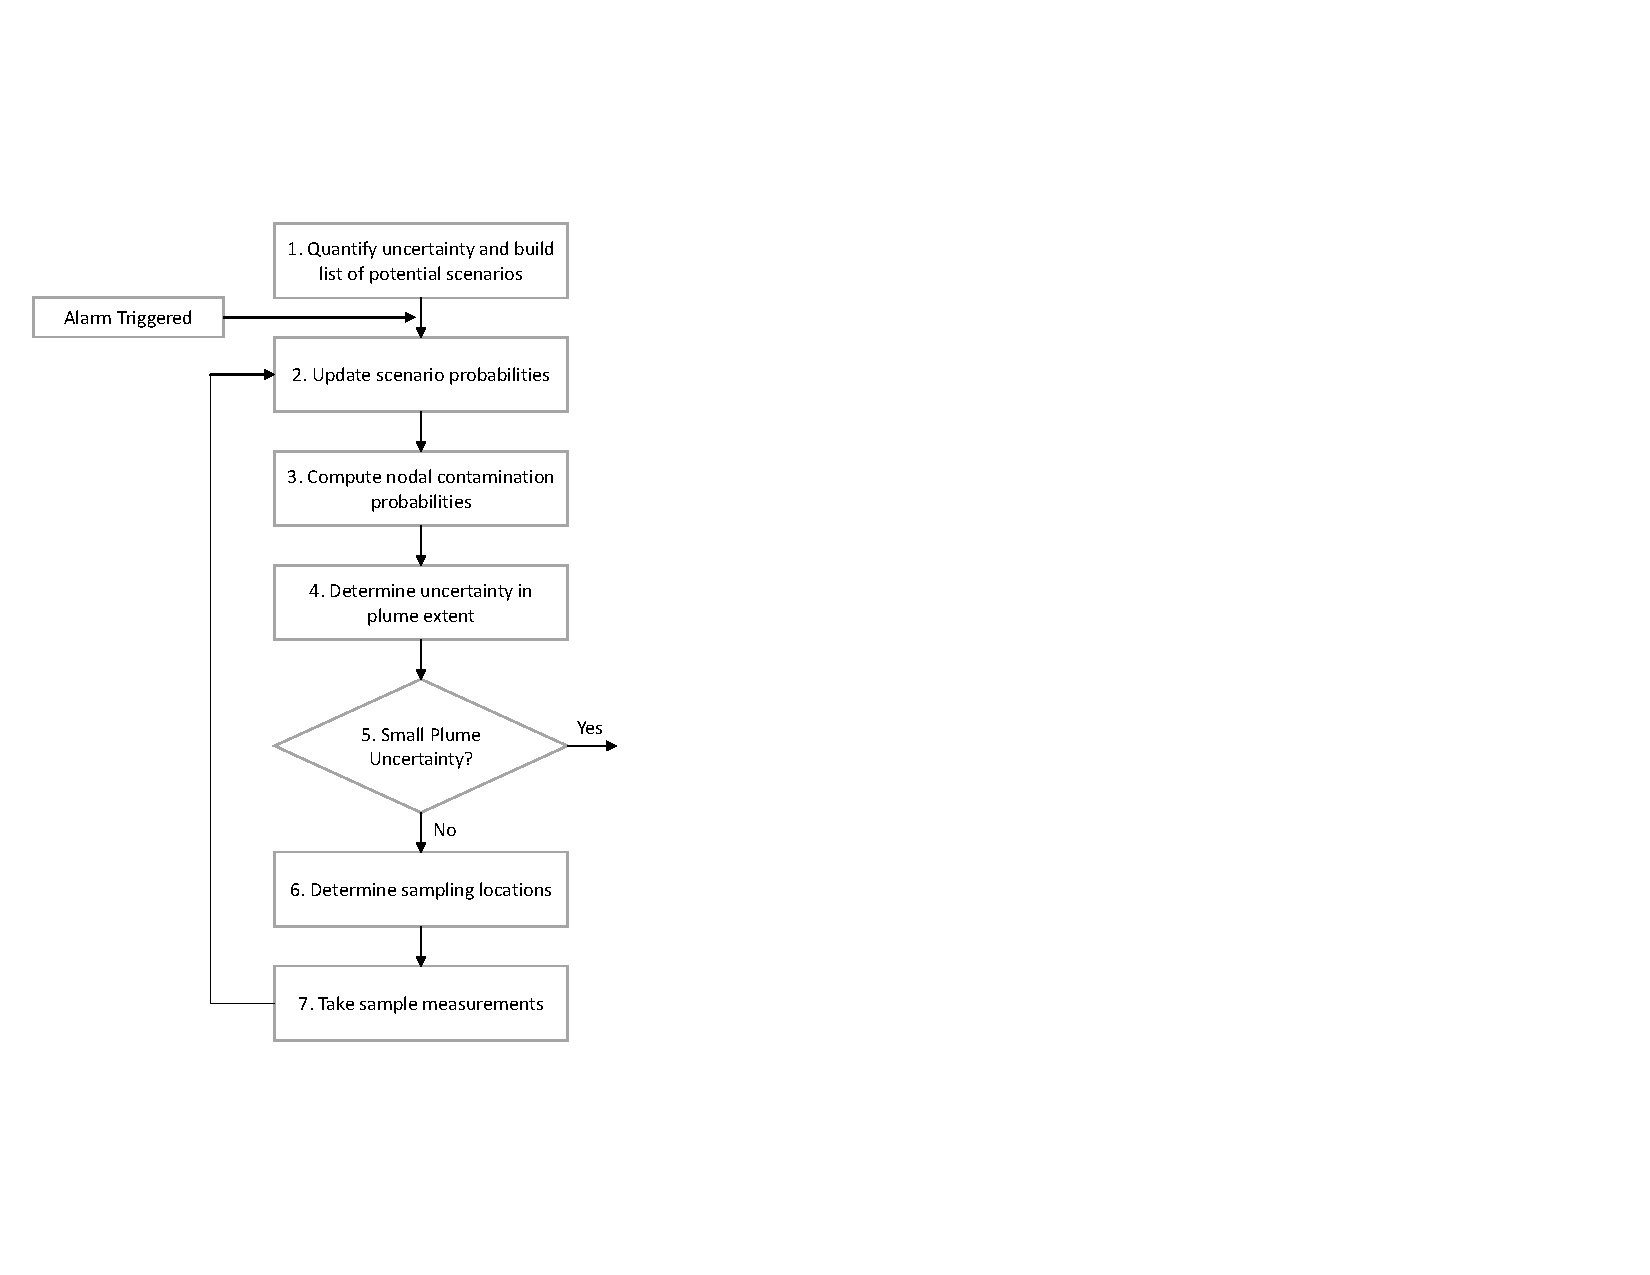
\includegraphics[scale=0.6]{graphics/uncertaintyprocess3.pdf}
\caption{Illustration of the source inversion and grab sample cycling strategy.}
\label{fig:ureduction_flowchart}
\end{center}
\end{figure}

\subsection{Case Study}
Since real system data is not available, the \code{measuregen}
executable is used again to generate simulated data for a contamination incident in the following case study.  In this simulation, 
a conservative contaminant is injected into node 115 of EPANET
Example Network 3 (Net3) at 8 am.  The set of potential scenarios includes 10 hydraulic realizations with 97 different injection locations. All of the files required 
for this case study are provided in the \code{examples/case\_studies/sampling} folder.
  
The case study is composed of four sampling cycles to reduce uncertainty in the extent of contamination. The initial warning is 
raised at 10 am. From this time, the procedure in Figure \ref{fig:ureduction_flowchart} is followed to reduce uncertainty by gathering 
grab samples every hour. In each sampling cycle, three additional samples are collected. Given the information provided by the new samples, 
the probability distribution of scenarios is updated following Bayesian statistics. Then, the methodology proposed in Section \ref{uqn_algorithms} 
is followed to quantify uncertainty. To facilitate the analysis, a script was implemented in Python to run the sampling cycles in a loop, which is the signals.py file provided in the \code{examples/case\_studies/sampling/cycling} folder. 
The execution of the script follows the same convention as the WST subcommands:

\begin{unknownListing}
python wst/packages/pywst/pywst/cycling/signals.py cycle <configfile>
\end{unknownListing}

The options for the script are the same as the options provided in the sections of the \code{inversion}, \code{uq} and \code{grabsample} subcommands. 
Some additional options to specify duration of each cycle and number of cycles are added. The configuration file for this case study, sampling\_case\_study.yml, 
is shown in Figure \ref{fig:case_study_conf}.  

\begin{figure}[!ht]
  \unknownInputListing{../../examples/case_studies/sampling/sampling_case_study.yml }{}{1}{13}
  \caption{The configuration file for sampling case study.}
  \label{fig:case_study_conf}
\end{figure}

\subsection{Cycle 0}
At 10 AM, the contamination warning system detects abnormal water quality at nodes 40 and 111. The measurement data from those two locations is used to 
perform a Bayesian update in the probability of scenarios. At this point, given the probability distribution of scenarios, 73 possible scenarios are 
identified as most likely. The uncertainty in the number of scenarios is evident in the uncertainty quantification as most of the nodes are deemed unknown (UN). 
Figure \ref{fig:case_study_cycle1} shows in yellow all locations that are considered uncertain to have contamination. 
The utility has three teams available to gather manual grab samples and it takes 60 minutes for each team to 
obtain the manual samples. The probability-based formulation in Chapter \ref{chap:grabsample} identifies the three optimal grab sample locations shown 
in dark gray/black in Figure \ref{fig:case_study_cycle1}.             

\subsection{Cycle 1}
At 11:00 AM, the new measurements are used to perform a Bayesian update and an uncertainty quantification. 
This time the number of uncertain nodes is reduced by half as shown in Figure \ref{fig:case_study_cycle2}. Nodes in red are likely to be contaminated (LY) and 
nodes in blue are likely to not be contaminated (LN). Again a 60-minute delay for sample collection and three sample teams were used in the probability-based 
formulation in Chapter \ref{chap:grabsample} to identify the optimal grab sample locations at 12:00 PM. The three new and three previous grab sample locations (dark gray/black) are shown in Figure \ref{fig:case_study_cycle2}.
        
\subsection{Cycle 2}
Grab sample measurements are obtained at 12:00 PM from the optimal locations identified in second cycle of the \code{grabsample} subcommand. 
These are used to perform Bayesian update and an uncertainty quantification again. 
Only seven nodes remain uncertain (UN) as to whether they are contaminated in this cycle. As the uncertainty is still not small enough, three more sampling locations are 
identified by solving the probability based formulation of Chapter \ref{chap:grabsample}. The three new grab sample locations plus the six previous (dark gray/black) are shown in 
Figure \ref{fig:case_study_cycle3}.

\subsection{Cycle 3}
Grab sample measurements are obtained at 1:00 PM from the optimal locations identified in in third cycle of the \code{grabsample} subcommand. 
With this new information, the Bayesian update and the uncertainty quantification lead to zero nodes classified as uncertain (all are likely yes or likely no). The three new grab sample locations plus the nine previous (dark gray/black) are shown in Figure \ref{fig:case_study_cycle4}. Only 11 grab sample locations are shown in this cycle since one of the locations was selected to be sampled twice, since different sampling times can provide different measurement data. 

\begin{figure}[!h]
\centering
\begin{subfigure}{0.49\textwidth}
\centering
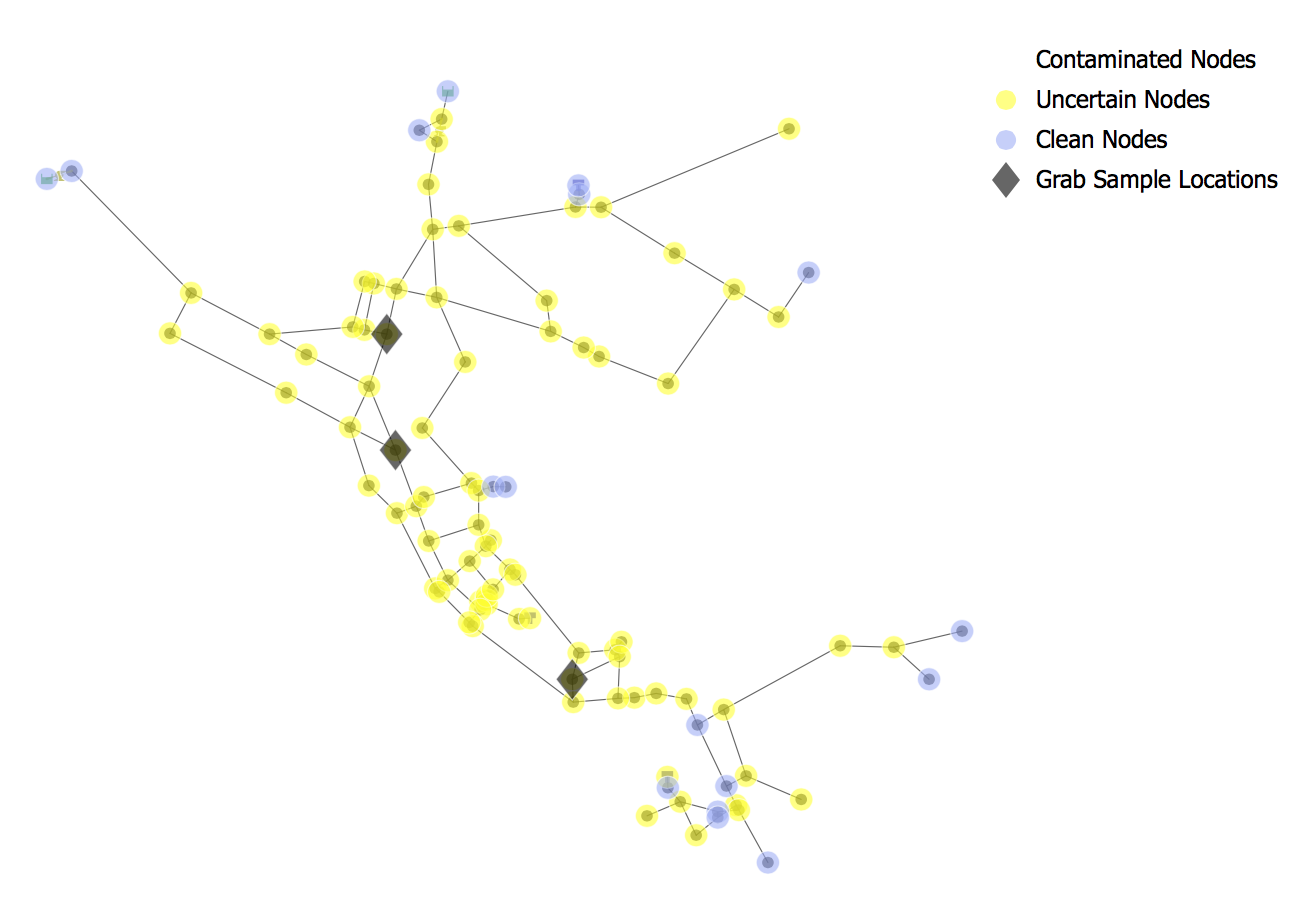
\includegraphics[width = \textwidth]{graphics/sampling_cs_cycle1.png}
\caption{Cycle 0}
\label{fig:case_study_cycle1}
\end{subfigure}
\begin{subfigure}{0.49\textwidth}
\centering
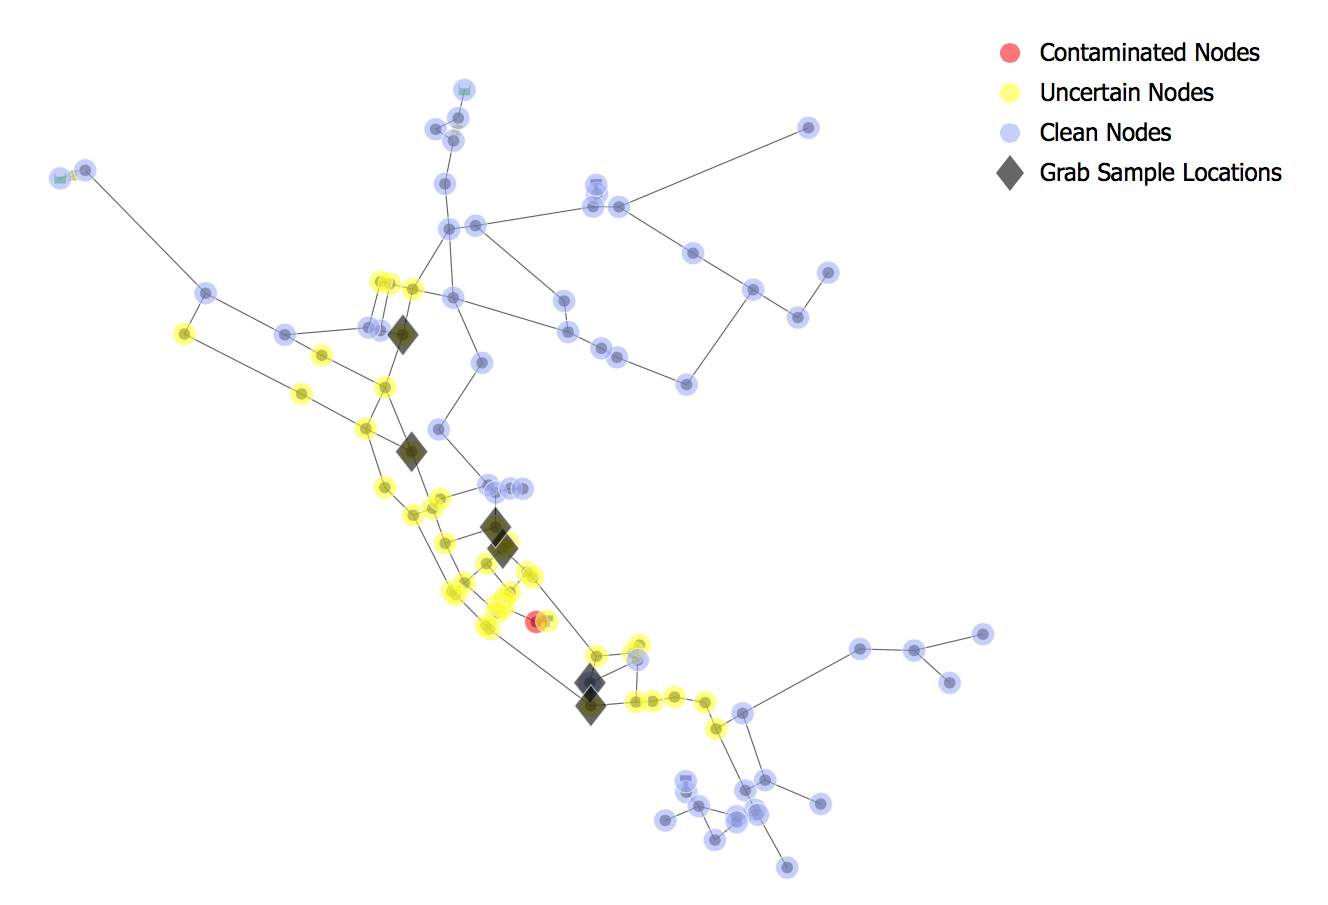
\includegraphics[width = \textwidth]{graphics/sampling_cs_cycle2.png}
\caption{Cycle 1}
\label{fig:case_study_cycle2}
\end{subfigure}
\centering
\begin{subfigure}{0.49\textwidth}
\centering
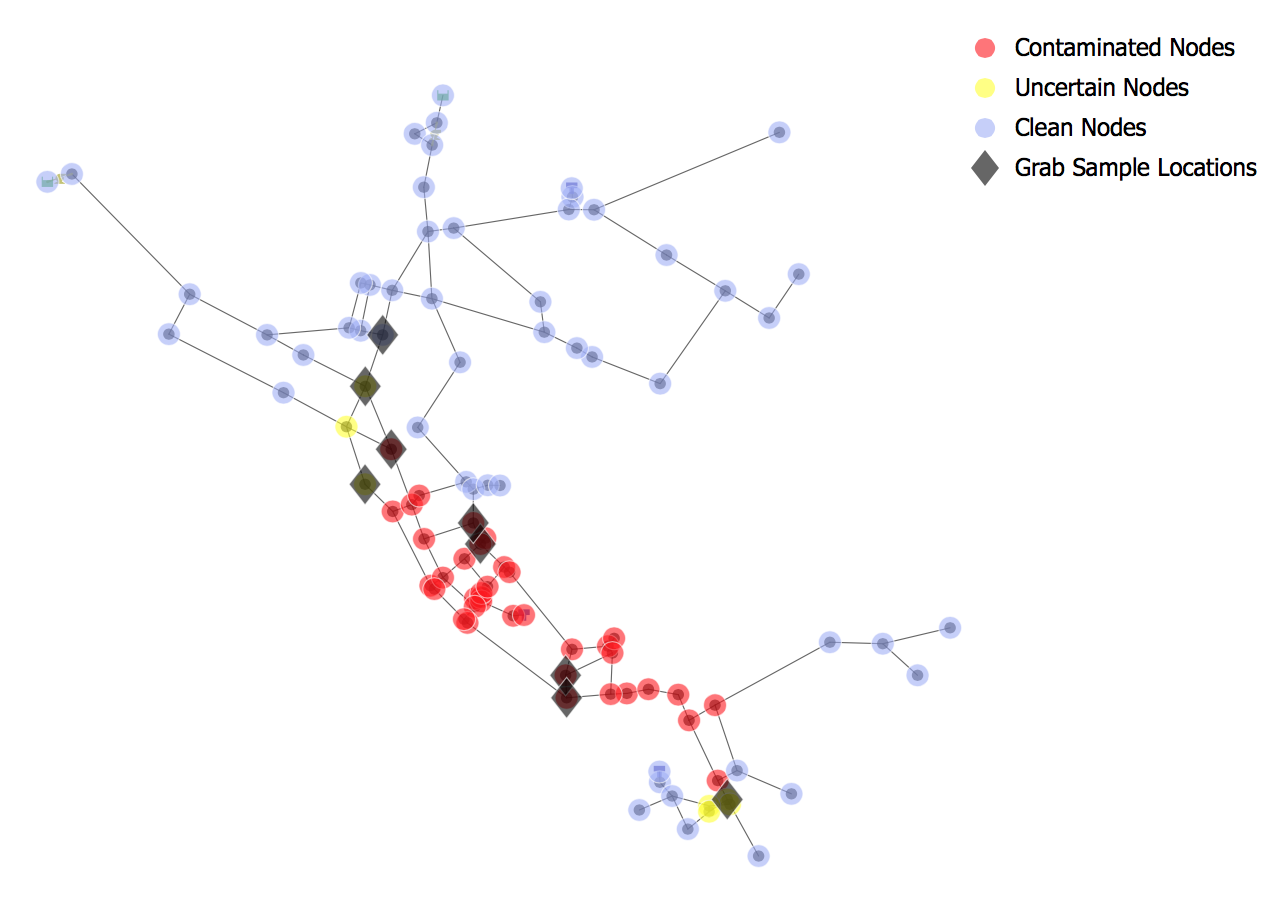
\includegraphics[width = \textwidth]{graphics/sampling_cs_cycle3.png}
\caption{Cycle 2}
\label{fig:case_study_cycle3}
\end{subfigure}
\begin{subfigure}{0.49\textwidth}
\centering
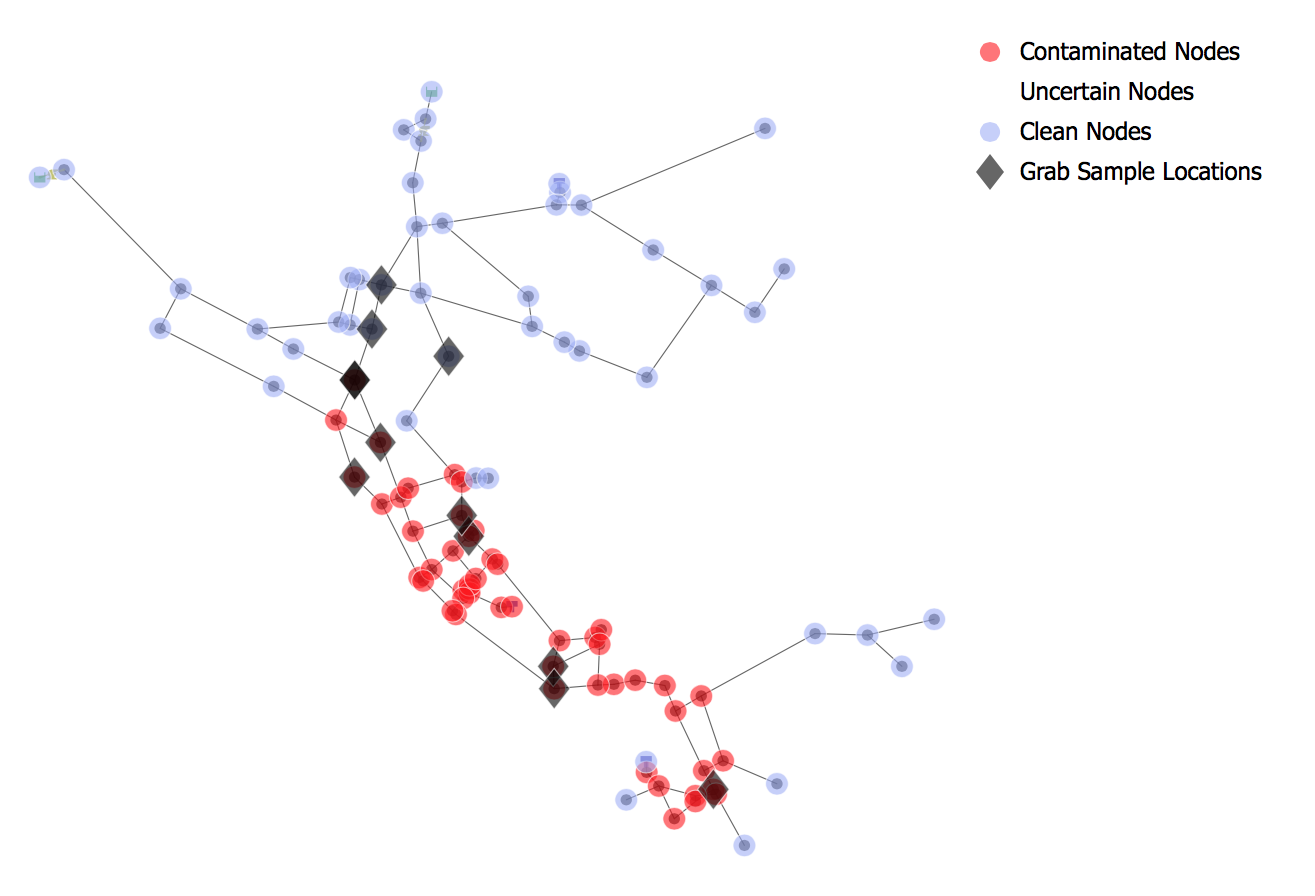
\includegraphics[width = \textwidth]{graphics/sampling_cs_cycle4.png}
\caption{Cycle 3}
\label{fig:case_study_cycle4}
\end{subfigure}
\caption{EPANET Example Network 3 with grab sample locations (dark gray/black diamonds), contaminated nodes (red circles), uncertain nodes (yellow circles), and clean nodes (blue-gray circles) identified for each of the cycles in the case study.}
\label{fig:gs_uq_case_study}
\end{figure}
